\clearpage
\section{各功能模块的 UI 界面及功能描述}

界面共 10 个：用户端 6 个（移动端 390$\times$844），管理后台 4 个（桌面端 1280$\times$820）。分两种尺寸是因为使用场景不同——学生在手机上碎片时间浏览与预约，管理员在电脑上批量审核与查日志，把管理功能塞进手机界面会为了适配小屏牺牲表格的对比效率。

设计遵循四条原则：状态可见（处在哪个状态、下一步能做什么一屏看清）、风险前置（不可逆操作前给出规则提示）、一屏一任务、两端一致（绿色可用、橙色注意、红色失败或违规）。主色 \#0E9F6E，价格色 \#F4511E，正文 \#16202B。8 个模块全部有界面承接，M8 公共支撑属于后端能力，以“消息”“图片上传”“超时自动完成提示”的形式出现在其他界面中。界面稿以 HTML/CSS 搭成可交互原型，按 2 倍分辨率导出为图片，10 个界面共用同一套颜色、字号、圆角与间距令牌。

\subsection{用户端界面}

\begin{center}
\begin{minipage}{0.97\textwidth}\centering
\begin{minipage}{0.41\linewidth}\centering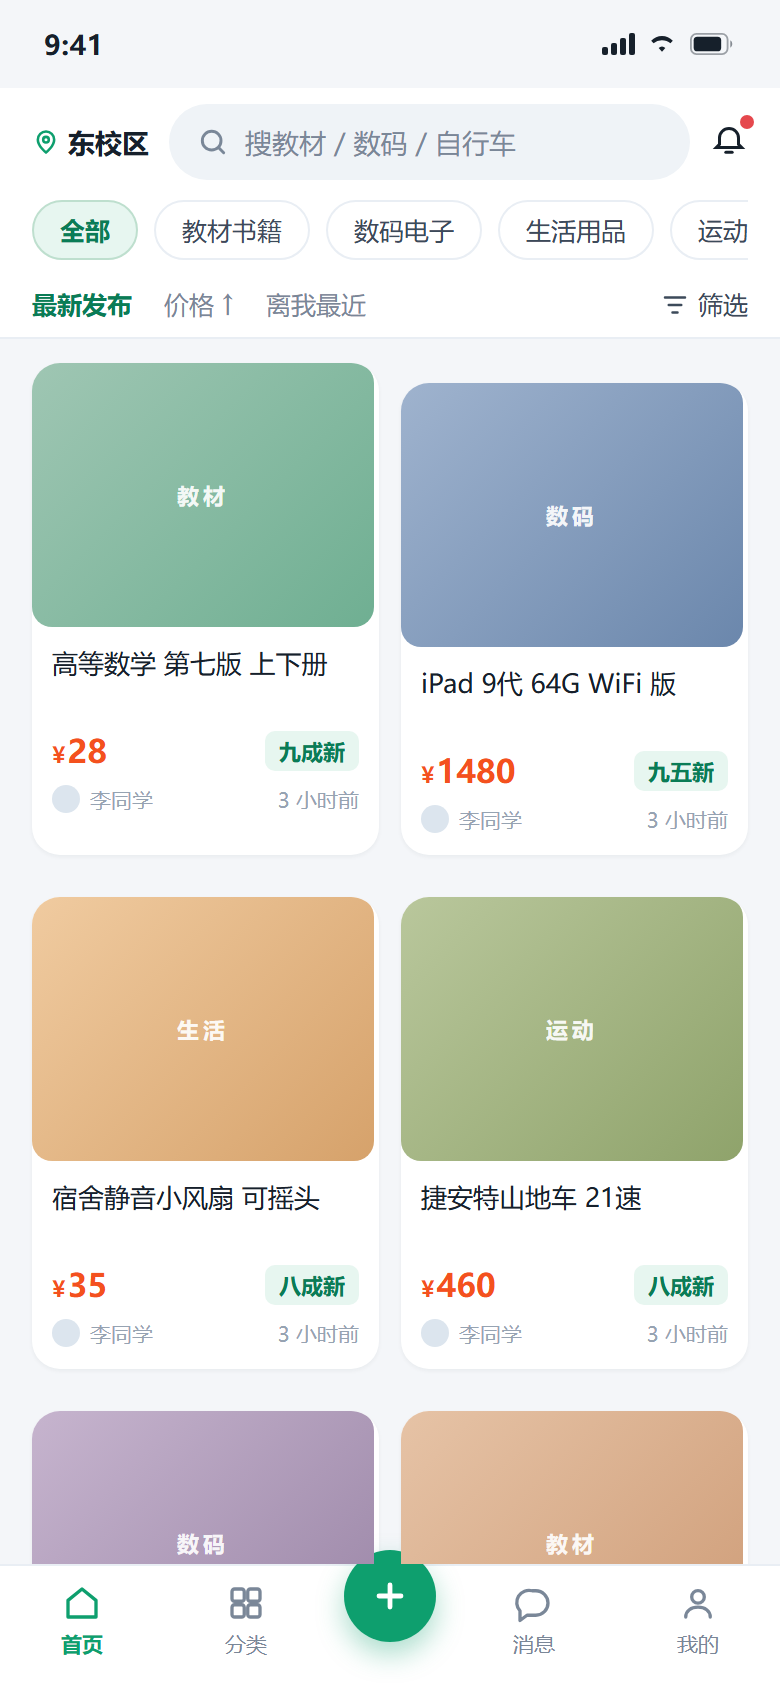
\includegraphics[width=\linewidth]{ui1.png}\end{minipage}\hfill
\begin{minipage}{0.41\linewidth}\centering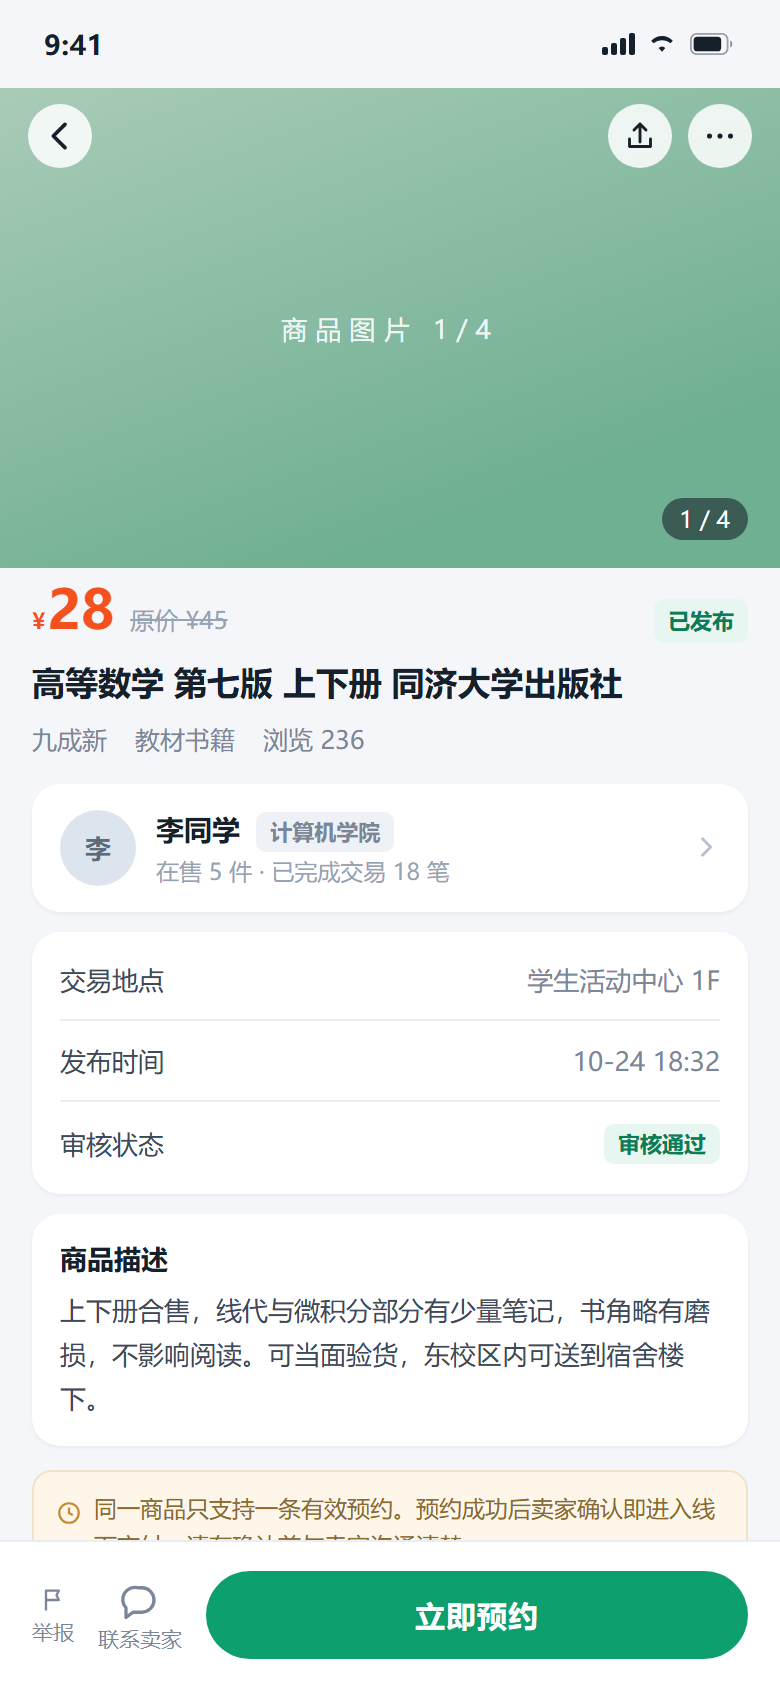
\includegraphics[width=\linewidth]{ui2.png}\end{minipage}
\par\vspace{2pt}
\captionof{figure}{界面 1 首页·商品查询（左）与界面 2 商品详情·预约（右）}\label{fig:ui12}
\end{minipage}
\end{center}

\textbf{界面 1}：顶部为位置、搜索框与消息入口，第二行分类快筛，第三行排序与筛选；商品以双列卡片呈现封面、标题、价格、成色、卖家与时间。公开列表只出现已发布商品，已预约、已确认、已完成、已下架的商品不在此出现（REQ-005）；成色用标签而非文字描述，便于扫视判断。

\textbf{界面 2}：大图区、价格与状态、卖家信息、交易地点与审核状态、商品描述，底部固定“举报 / 联系卖家 / 立即预约”。价格区直接标注“已发布”，用户不必猜商品是否还能预约；底部提示条写明“同一商品只支持一条有效预约”，把 REQ-001 的规则前置到操作之前；商品已被预约时按钮替换为不可点击的“已被预约”。

\begin{center}
\begin{minipage}{0.97\textwidth}\centering
\begin{minipage}{0.41\linewidth}\centering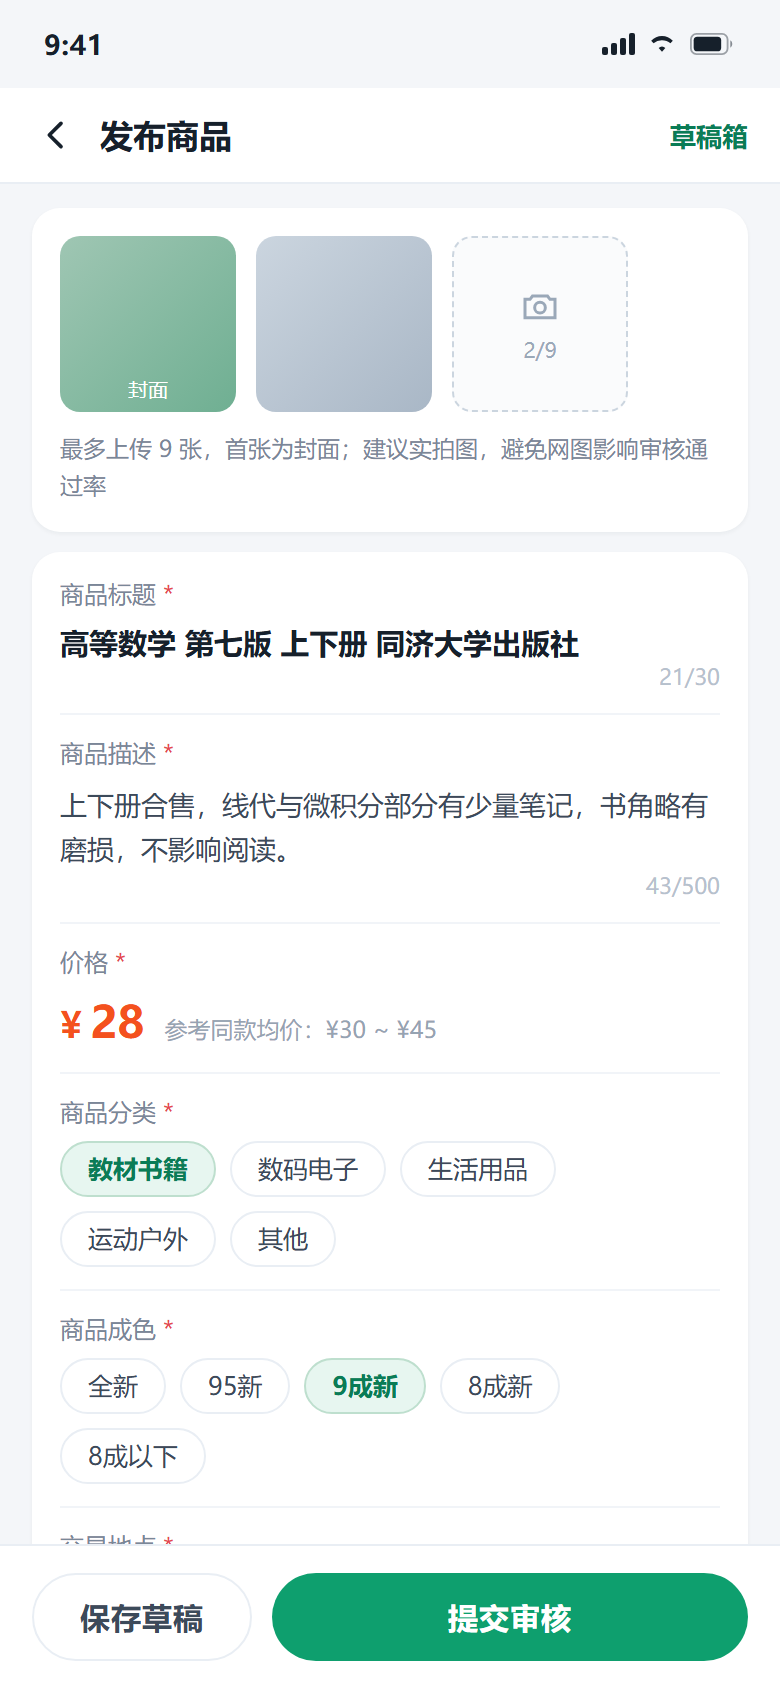
\includegraphics[width=\linewidth]{ui3.png}\end{minipage}\hfill
\begin{minipage}{0.41\linewidth}\centering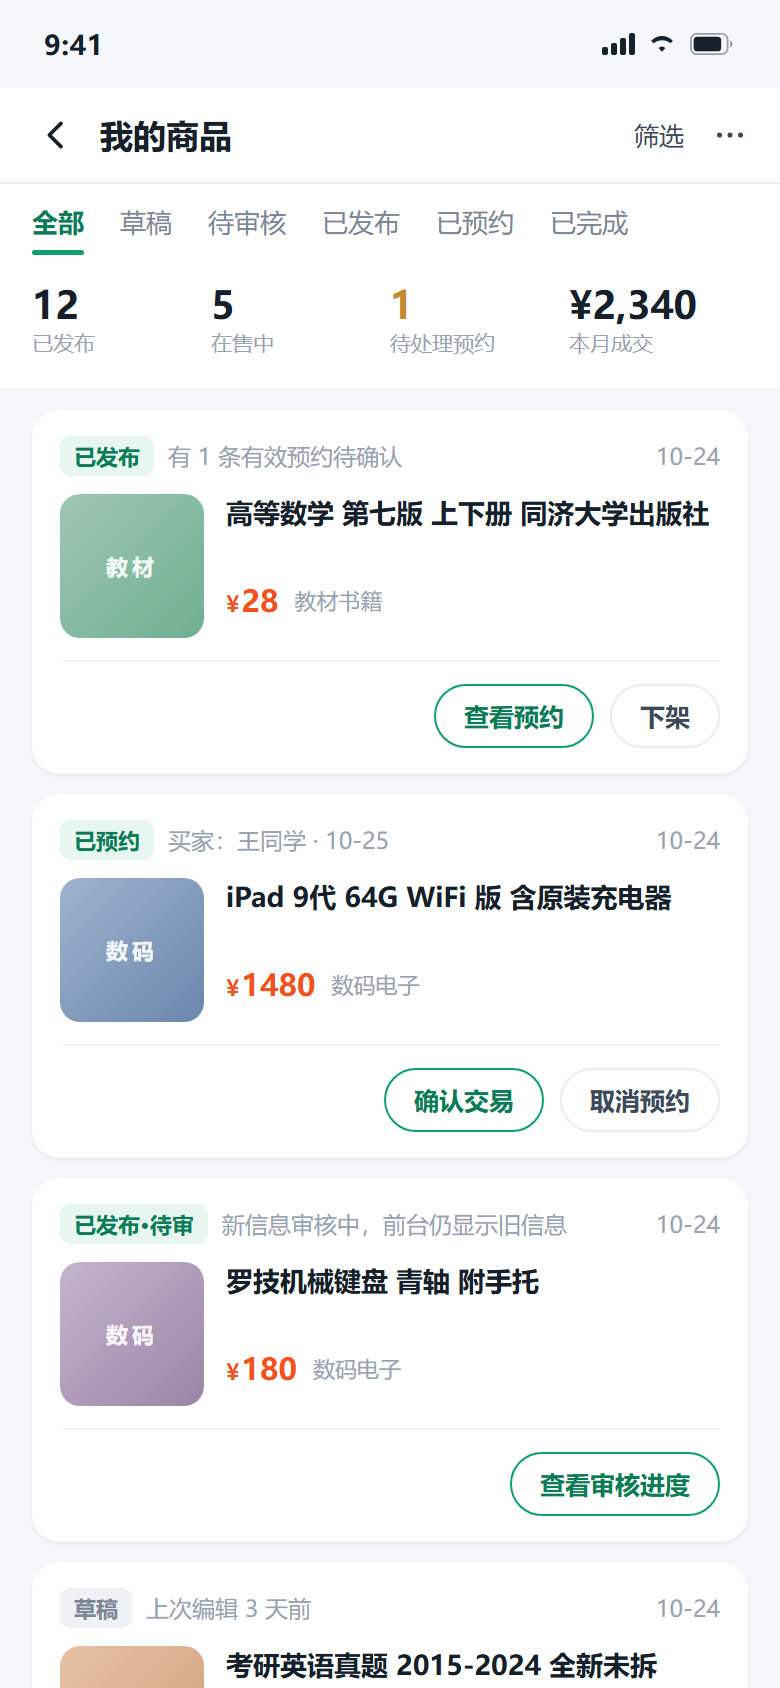
\includegraphics[width=\linewidth]{ui4.png}\end{minipage}
\par\vspace{2pt}
\captionof{figure}{界面 3 发布商品（左）与界面 4 我的商品（右）}\label{fig:ui34}
\end{minipage}
\end{center}

\textbf{界面 3}：九宫格图片上传（首张为封面）、标题、描述、价格、分类、成色、交易地点，必填项用红色星号标注，价格下方给出同款均价。提示条说明“提交后进入审核队列，审核通过前不会出现在公开列表”，把审核流程透明化；底部“保存草稿”与“提交审核”并列，对应 REQ-002 的两种保存方式。

\textbf{界面 4}：顶部按状态分栏，下方四个统计数字，列表项以状态标签开头，右侧只给出当前状态允许的操作。这是“组合状态”唯一能被用户看见的地方——第三个商品显示“已发布·待审”，说明新内容在审核、前台仍展示旧信息（REQ-017）；“确认交易 / 取消预约”只出现在已预约商品上，“下架”只出现在已发布商品上，按钮与状态严格绑定。

\begin{center}
\begin{minipage}{0.97\textwidth}\centering
\begin{minipage}{0.41\linewidth}\centering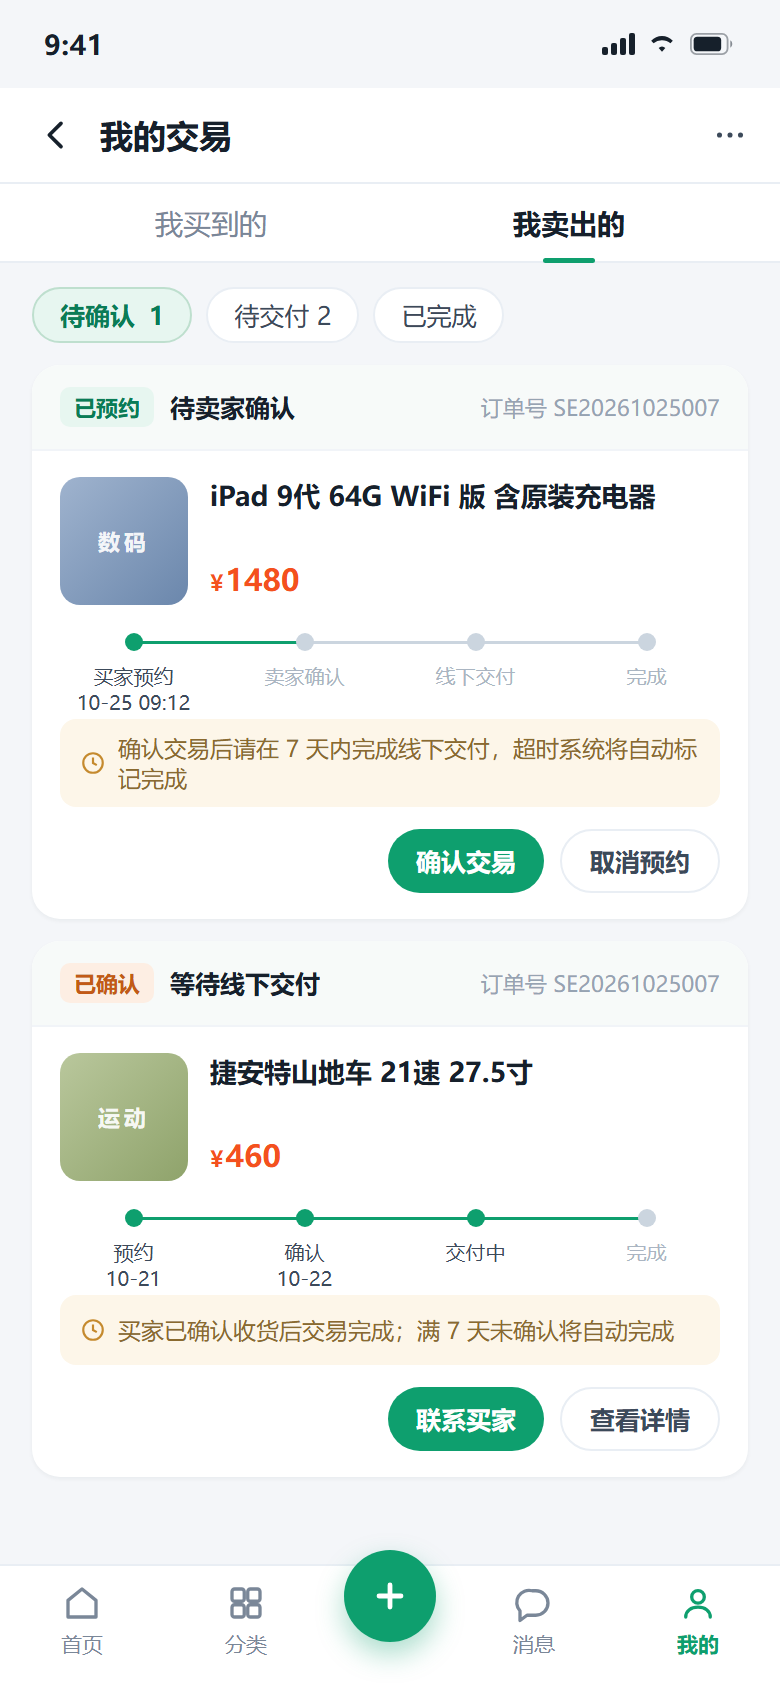
\includegraphics[width=\linewidth]{ui5.png}\end{minipage}\hfill
\begin{minipage}{0.41\linewidth}\centering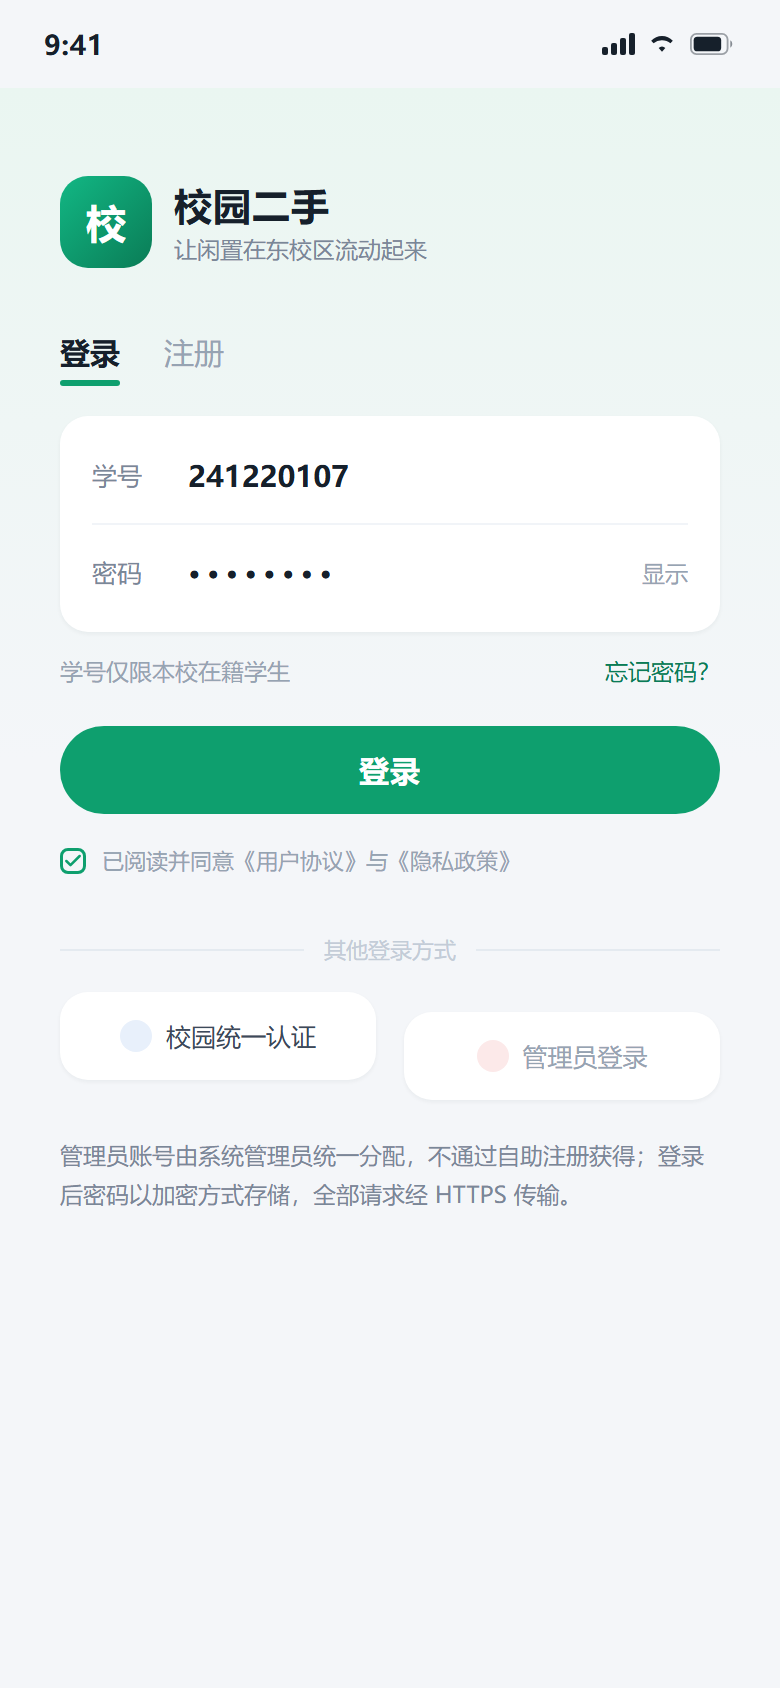
\includegraphics[width=\linewidth]{ui6.png}\end{minipage}
\par\vspace{2pt}
\captionof{figure}{界面 5 我的交易（左）与界面 6 登录 / 注册（右）}\label{fig:ui56}
\end{minipage}
\end{center}

\textbf{界面 5}：分“我买到的”与“我卖出的”两个视角，本图为卖家视角。每张卡片包含状态条、商品信息、四段式进度条（预约—确认—交付—完成）、提示条与操作按钮。进度条让用户一眼看出卡在哪一步；提示条写明“确认后请在 7 天内完成交付，超时系统将自动标记完成”，让 REQ-015 的自动行为可预期，买家视角在同一位置显示倒计时。

\textbf{界面 6}：品牌区、登录/注册切换、学号与密码、协议勾选、其他登录方式。账号字段直接写“学号”并注明“仅限本校在籍学生”，从入口避免重复账号；管理员登录单独作为入口并注明由系统统一分配，对应 REQ-004；页面底部说明密码加密存储与全站 HTTPS，把 REQ-012 的安全约定告知用户。

\subsection{管理后台界面}

\begin{center}
\begin{minipage}{0.80\textwidth}\centering
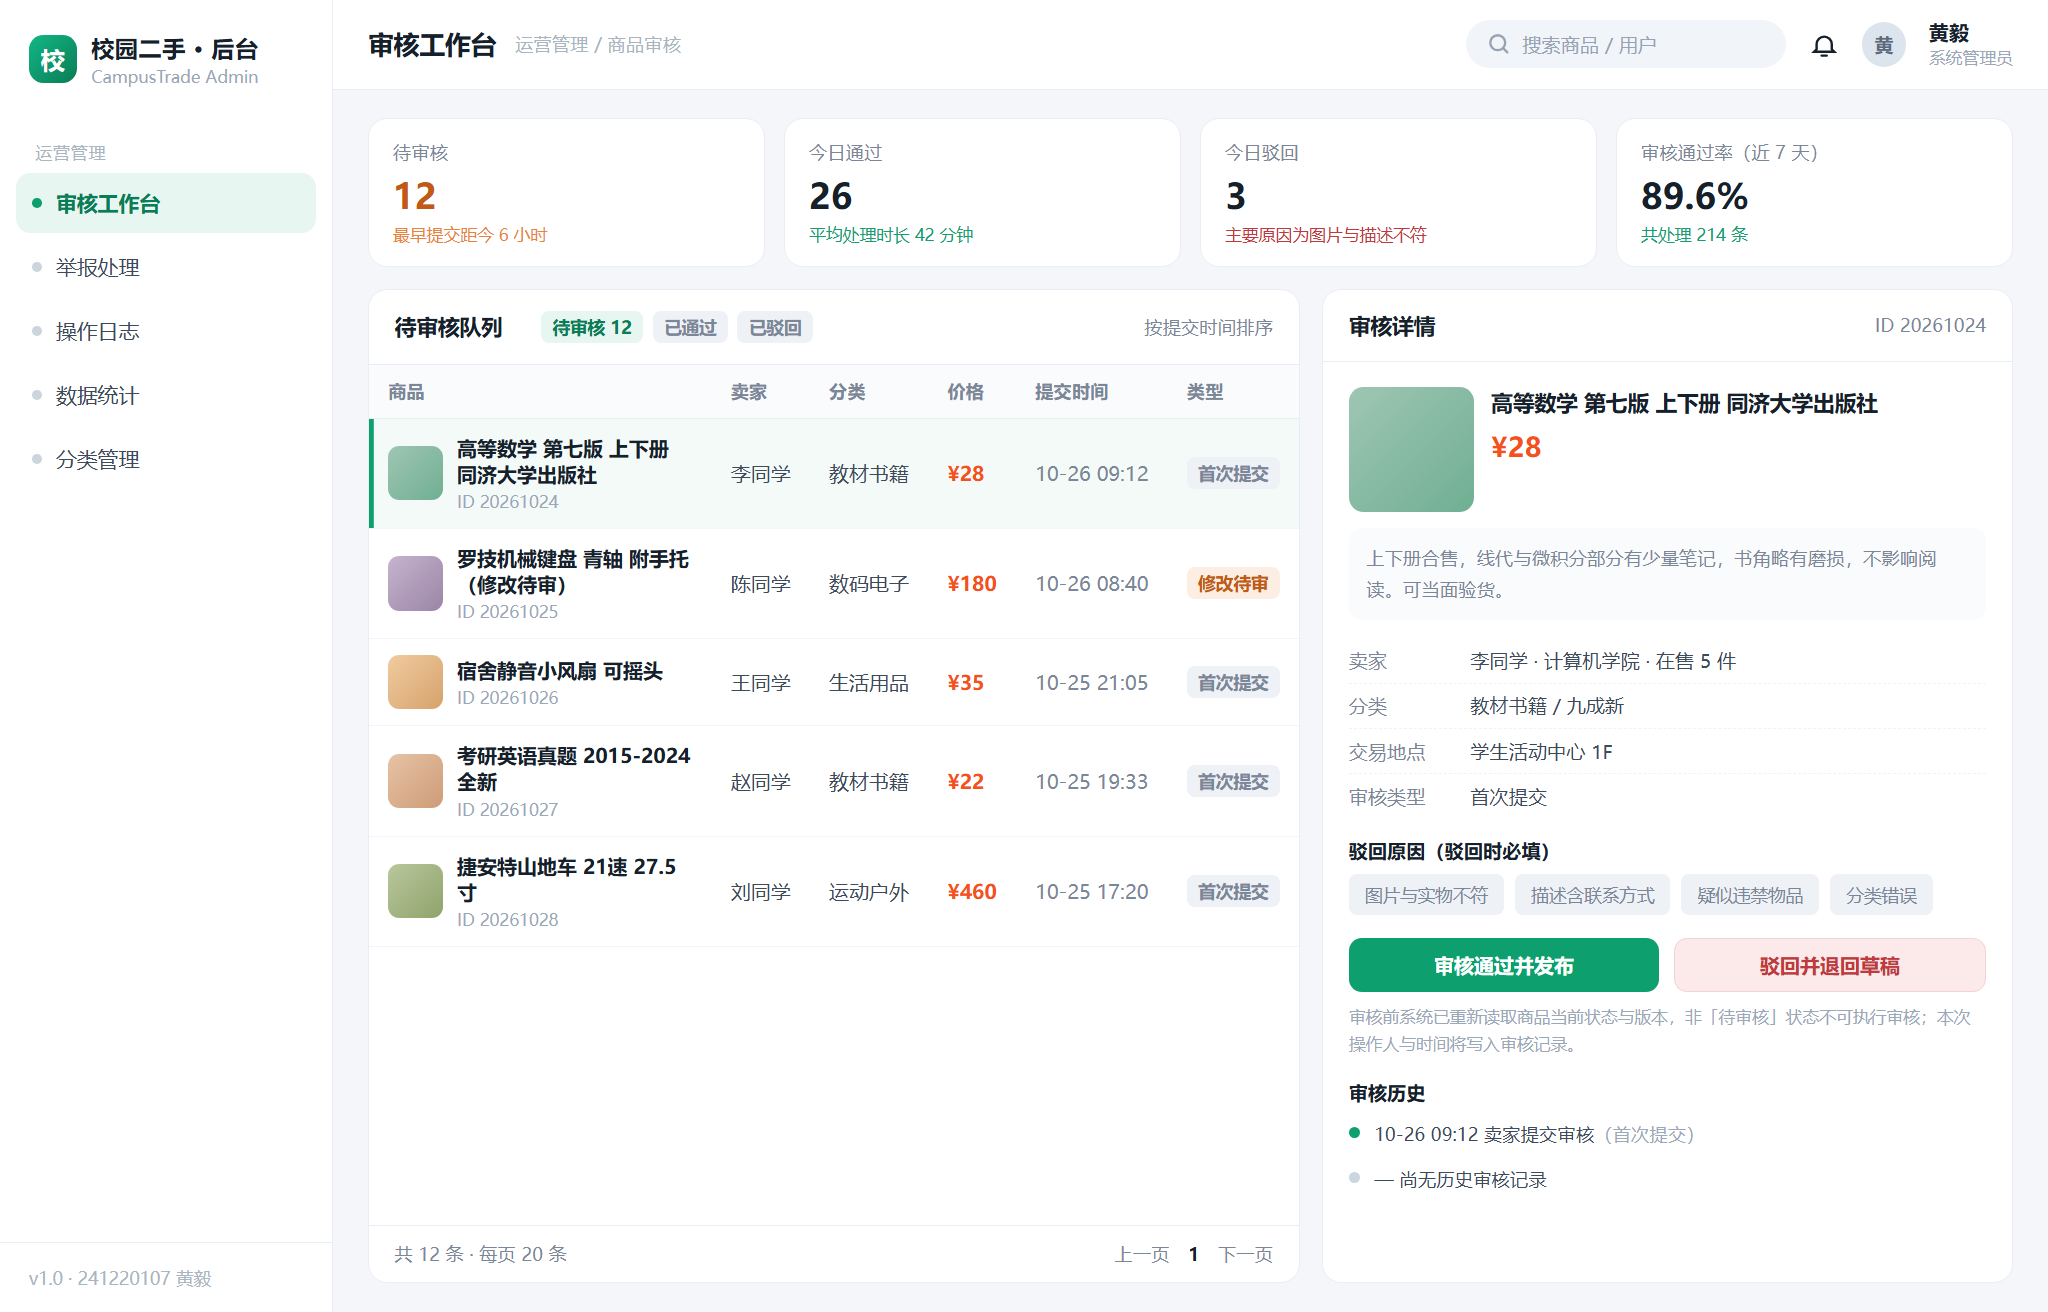
\includegraphics[width=\linewidth]{ui7.png}
\par\vspace{2pt}
\captionof{figure}{界面 7 审核工作台}\label{fig:ui7}
\end{minipage}
\end{center}

顶部指标卡与左侧待审核队列配合使用；驳回原因做成可点选标签而非自由输入，保证原因可统计；按钮下方注明“审核前已重新读取商品状态与版本”，把 REQ-003 的并发处理写在界面上；底部固定展示审核历史，首次提交也显示“尚无记录”。

\begin{center}
\begin{minipage}{0.80\textwidth}\centering
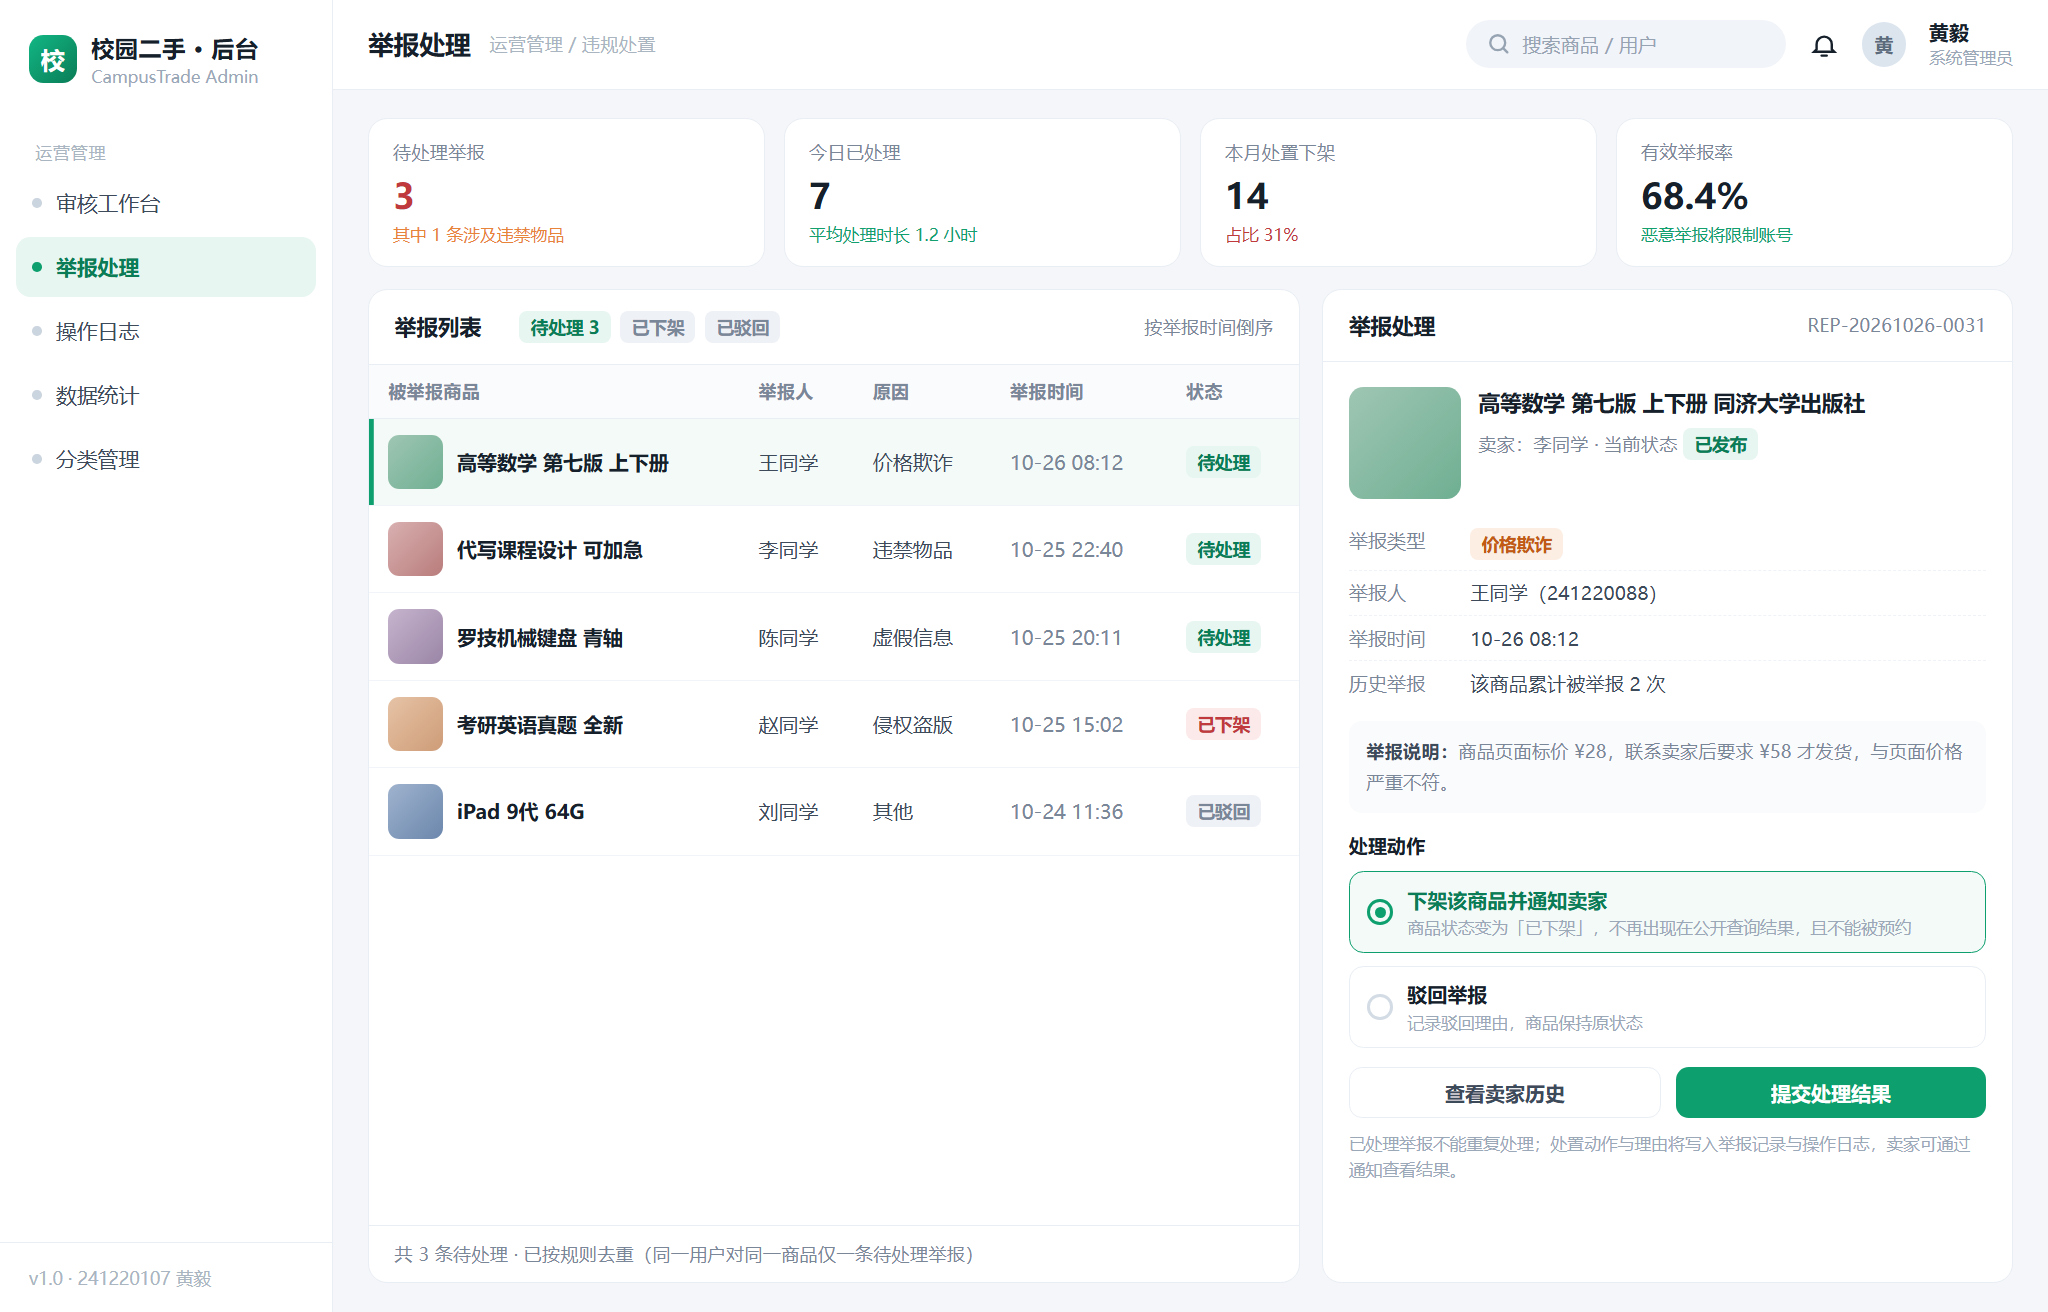
\includegraphics[width=\linewidth]{ui8.png}
\par\vspace{2pt}
\captionof{figure}{界面 8 举报处理}\label{fig:ui8}
\end{minipage}
\end{center}

结构与审核工作台一致。处置动作以单选卡片呈现并展开说明后果（“商品变为已下架，不再出现在查询结果，且不能被预约”），避免不清楚影响就点下架；面板显示累计被举报次数，为判断恶意卖家提供依据。

\begin{center}
\begin{minipage}{0.80\textwidth}\centering
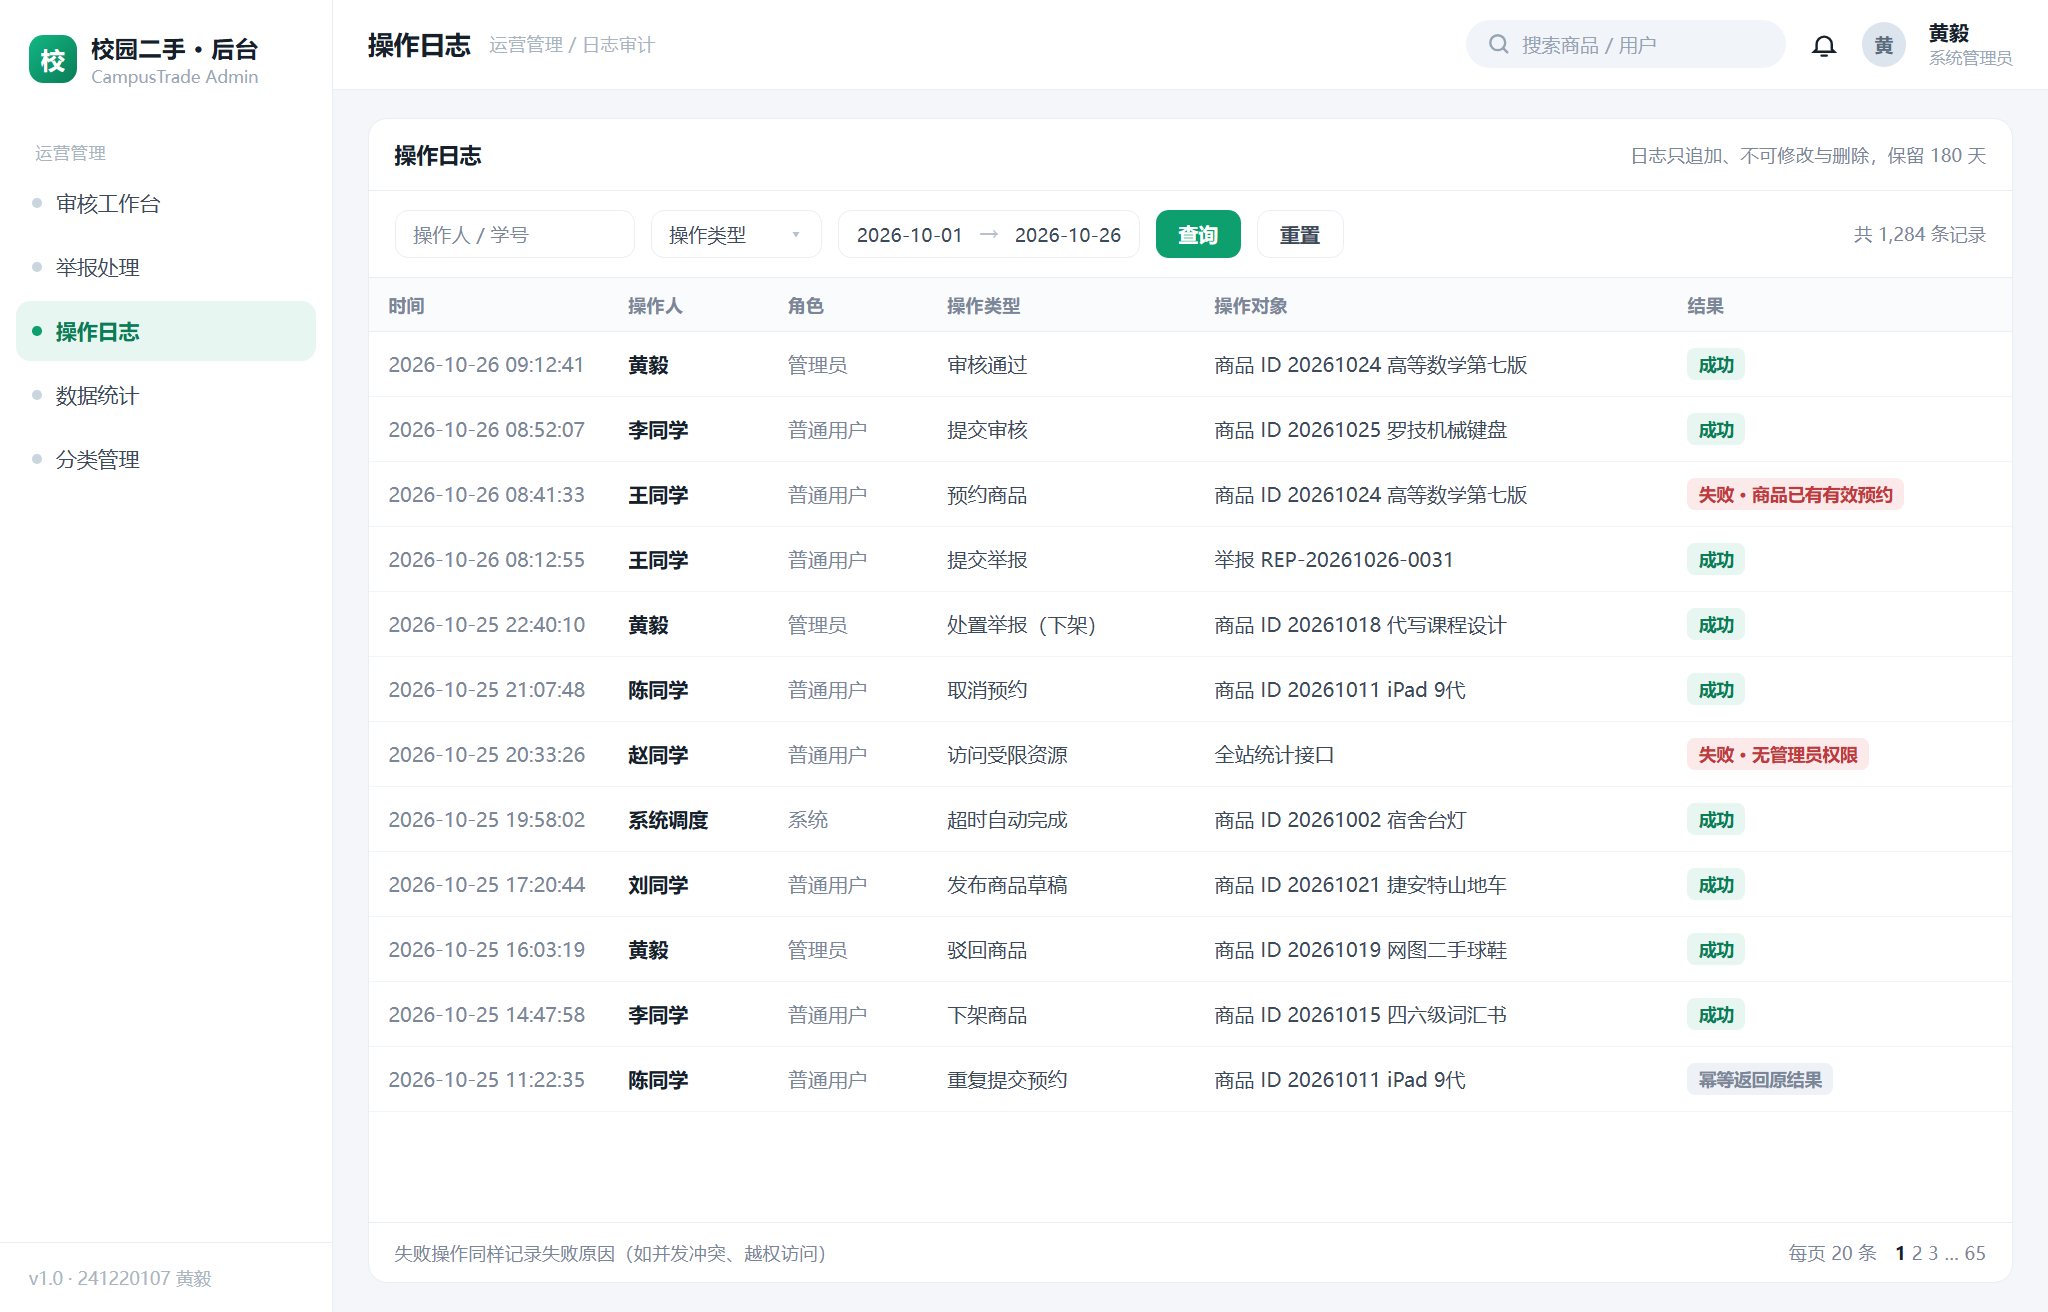
\includegraphics[width=\linewidth]{ui9.png}
\par\vspace{2pt}
\captionof{figure}{界面 9 操作日志查询}\label{fig:ui9}
\end{minipage}
\end{center}

顶部为查询条件（操作人、类型、时间范围），中间为日志表格。结果列含成功与失败，失败项用红色标签写明原因（“失败·商品已有有效预约”“失败·无权限”），对应 REQ-013 的“失败也记录”；顶部标注“只追加、不可修改与删除”。

\begin{center}
\begin{minipage}{0.80\textwidth}\centering
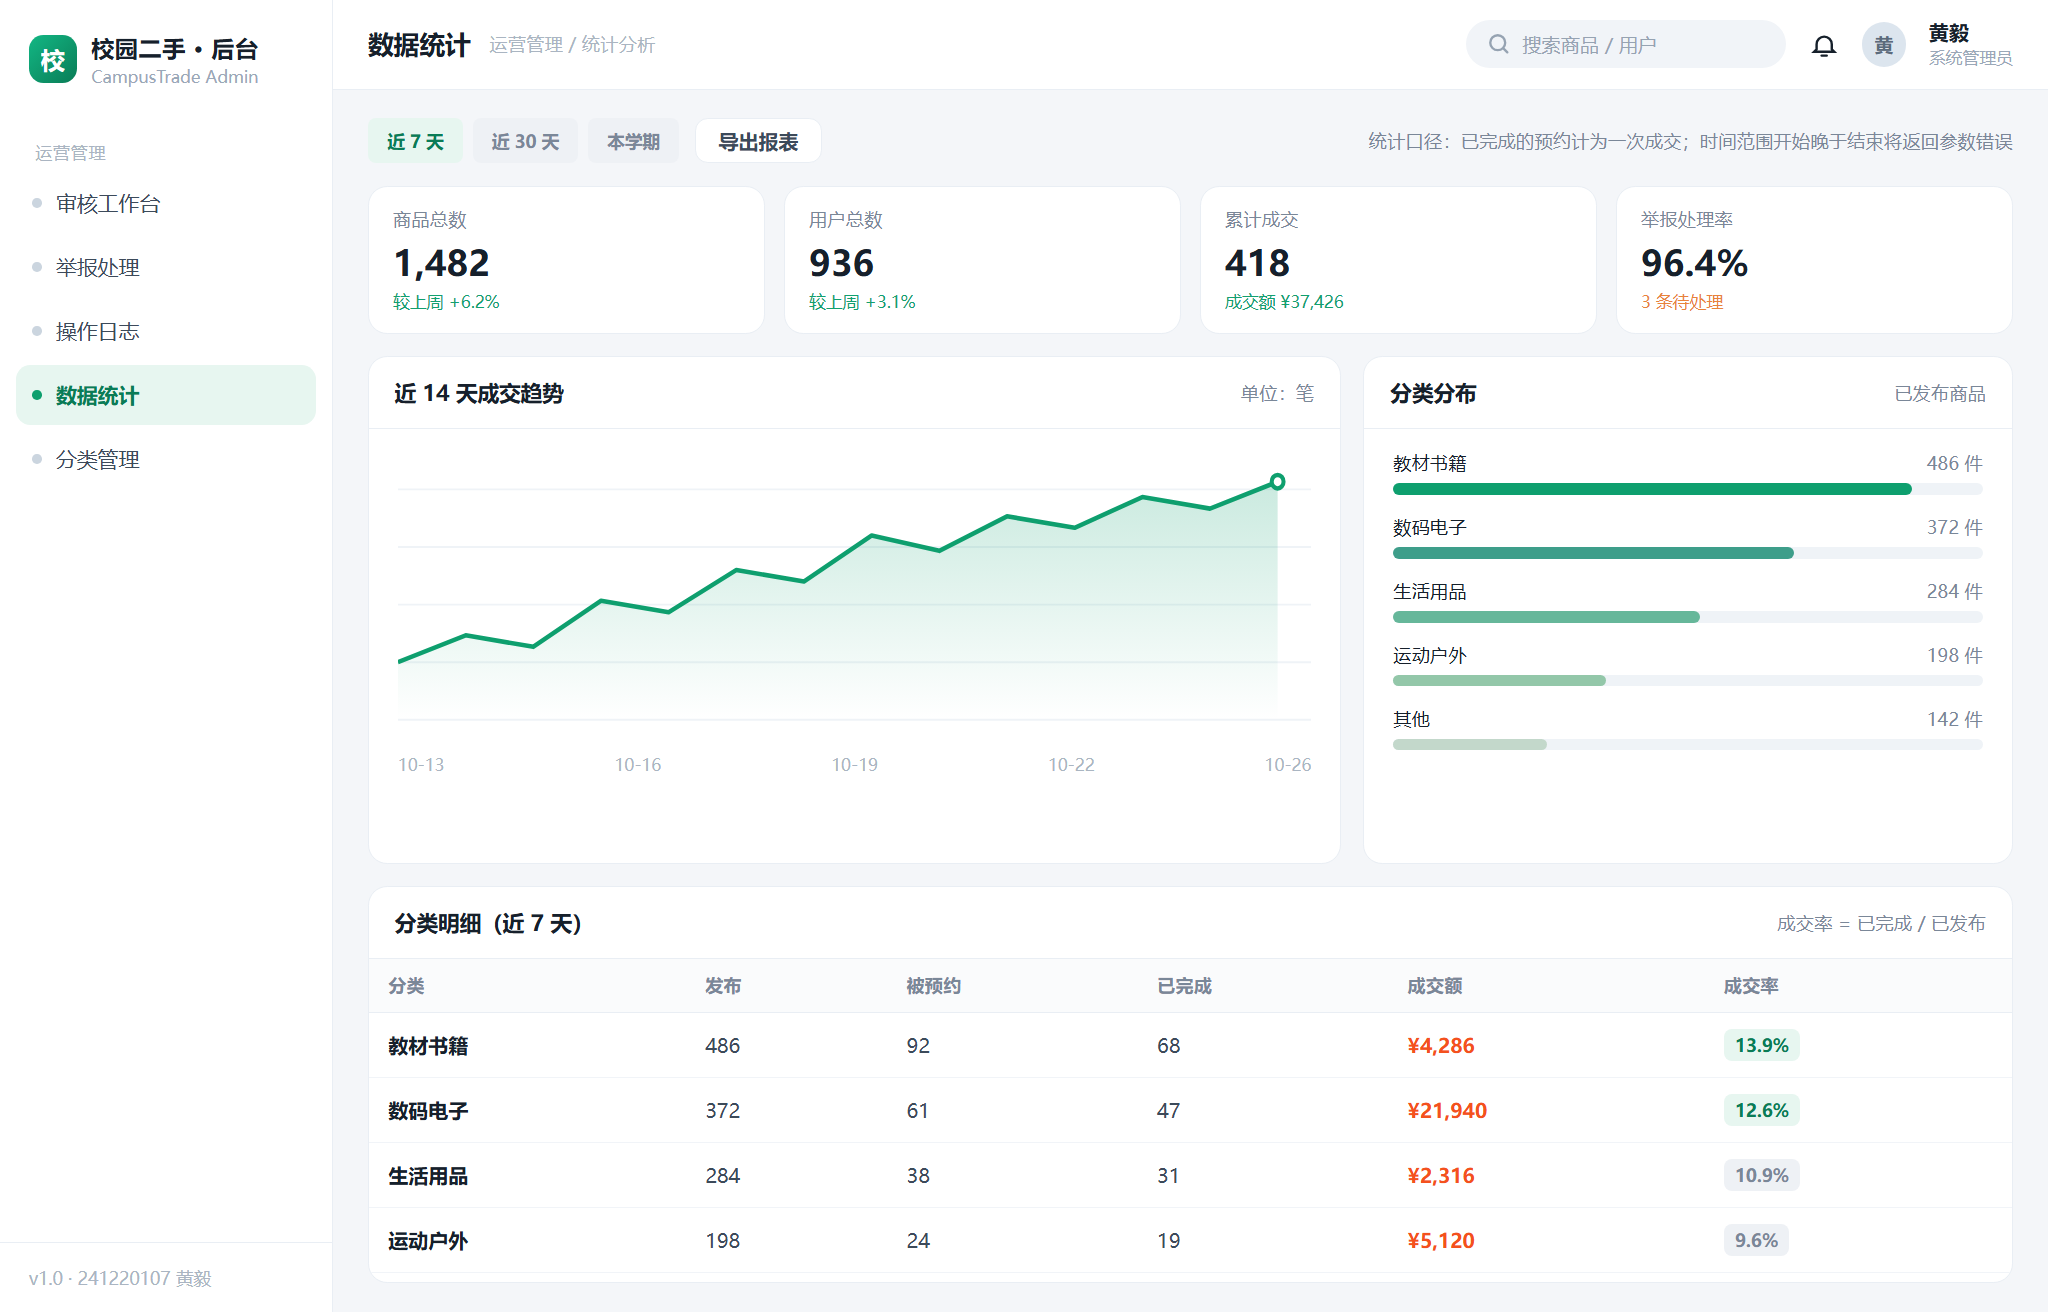
\includegraphics[width=\linewidth]{ui10.png}
\par\vspace{2pt}
\captionof{figure}{界面 10 数据统计}\label{fig:ui10}
\end{minipage}
\end{center}

时间范围切换与导出、四个指标卡、成交趋势、分类分布与明细表。顶部写明口径“已完成的预约计为一次成交”，并提示“时间范围开始晚于结束将返回参数错误”（REQ-018）；卖家视角复用同一页面，范围换成本人。
